\documentclass[
	doc,
	a4paper,
	helv
	]{apa6}
\usepackage[ngerman]{babel}
\usepackage[T1]{fontenc}
\usepackage[utf8]{inputenc}

\setcounter{secnumdepth}{3}

\geometry{
	left=2.5cm,
	right=2cm,
	top=2cm,
	bottom=2cm
	}
\usepackage[onehalfspacing]{setspace}

\usepackage{lmodern}
\usepackage{microtype}

\usepackage{tabularx}
\usepackage{siunitx}
\usepackage{eurosym}

\usepackage{xcolor}
\usepackage{hyperref}
\hypersetup{
		colorlinks	= true,
		linkcolor	= black,
		urlcolor	= blue,
		citecolor	= blue,
		pdftitle    = {Enterprise Architecture Management},
  		pdfsubject  = {Enterprise Architecture Management},
  		pdfauthor   = {Panagiota Sismanidou},
  		pdfkeywords = {Enterprise Architecture Management} ,
  		pdfcreator  = {pdflatex},
  		pdfproducer = {LaTeX with hyperref}
	}

\usepackage{csquotes}
\usepackage[
	style=apa,
	sortcites=true,
	sorting=nyt,
	backend=biber
	]{biblatex}
\DeclareLanguageMapping{german}{german-apa}
\addbibresource{Literaturverzeichnis.bib}

\title{Enterprise Architecture Management}
\shorttitle{EAM in der Praxis}
\author{Panagiota Sismanidou}
\leftheader{Simanidou}
\twoaffiliations{FOM Düsseldorf - IT Management}{Prof. Dr. Oliver Linssen}
%\abstract{}
\keywords{Enterprise Architecutre Management, Regierungssektor, Bankensektor, Bildungssektor}



\begin{document}
\maketitle

\newpage
\tableofcontents

\newpage

\section{Einführung in Enterprise Architecture Management}

Bis zu vorherigem Zeitpunkt erforderten Computermanipulationsverfahren keine derart ausgefeilten Managementstrategien. Heute implementieren Unternehmen neue Technologien, um die Struktur von Unternehmen zu organisieren und einen strategischen Vorteil zu erlangen, weil diese Verfahren im Laufe der Zeit immer komplexer werden.

In der ersten Phase der Business-Integration und IT (ab Mitte der 80er Jahre bis Mitte der 90er Jahre) war es unmöglich, die Automatisierung von Geschäftsprozessen zu realisieren, die auch in der Vor-Computer-Ära existierte.

Die zweite Phase (von Mitte der 1990er bis Mitte der 2000er Jahre) ist die Neuorganisation von Geschäftsprozessen. Es wurde davon ausgegangen, dass die Architekten des Informationssystems eine neue Geschäftsorganisationsstruktur anbieten würden, die mit der IT so kompatibel wie möglich ist. Dieser Zeitraum fiel mit der Begeisterung für ERP-Systeme und Geschäftsprozessmodellierungswerkzeuge zusammen. 

Heutzutage, wo neue Produkte und Anwendungen auf dem Markt Platz nehmen, steigen die Anforderungen an die Anpassungsfähigkeit von Unternehmen jedes Jahr. Es besteht die Notwendigkeit für viele makroökonomische Indikatoren zu einer noch umfassenderen Konsolidierung der verschiedenen  Bereiche eines Unternehmens oder einer Organisation durch den Einsatz elektronischer Werkzeuge.

\subsection{Enterprise Architecture Management Definition}
Als eine Lösung für das Problem der Anpassungsfähigkeit neuer Technologien in der Struktur eines Unternehmens ist das Enterprise Architecture Management (EAM). EAM hilft dabei, alle Funktionen innerhalb der Organisation zu synchronisieren und initiiert gleichzeitig einen Zyklus kontinuierlicher Änderungen für die Zwecke der Geschäftsoptimierung. Es gibt keine einheitliche Definition in der Literatur, denn jeder Autor beschreibt die Bedeutung des EAM anders. Eine sinnvolle Definition, die ausführlich das EAM beschreibt, ist folgende:

\begin{quote}
\glqq Enterprise Architecture Management ist ein systematischer und ganzheitlicher Ansatz für das Verstehen, Kommunizieren, Gestalten und Planen der fachlichen und technischen Strukturen im Unternehmen. Es hilft dabei, die Komplexität der IT-Landschaft zu beherrschen und die IT-Landschaft strategisch und businessorientiert  weiterzuentwickeln.\grqq
\autocite{Hanschke2016}
\end{quote}

EAM ist ein wesentlicher Bestandteil des strategischen IT-Managements und beinhaltet alle Prozesse für die Dokumentation, Analyse, Qualitätssicherung, Planung und Steuerung der Weiterwicklung der IT-Landschaft und der Geschäftsarchitektur. Es stellte sich jedoch heraus, dass das moderne Geschäft eine sehr mobile Struktur darstellt und sich ständig verändern muss, um seine Position auf dem Markt zu halten. EAM findet sich hauptsächlich in großen Organisationen -- je großer ein Unternehmen ist, desto komplexer ist die IT-Infrastruktur. Darüber hinaus sind große Unternehmen auf einem höheren Niveau der Reife angeordnet (basierend Reifemodell des Unternehmens von der Carnegie Mellon University \textcolor{red}{(Quelle?)}) Die Einführung von Managementsystemen Architektur stellt das höchste Niveau der Reife dar.

Nach Angaben der Internationalen Vereinigung der CFOs, Beiträgen der Zeitschrift Business Week und der Analysten Ernst \& Young zeigen Best Practice-Beispiele, dass große Unternehmen im ersten Jahr nach Einführungvon EAM-Systemen Verbessrungen bringen, die Millionen Dollar einsparen können.
%εξασφαλίζοντας ότι οι βέλτιστες πρακτικές και τα πρότυπα σε μια μεγάλη εταιρεία κατά το πρώτο έτος λειτουργίας του ΕΑΜ-συστημάτων μπορεί να φέρει αποτέλεσμα, το οποίο μετράται σε εκατομμύρια δολάρια.
Nach Deloitte, können durch die  korrekte Beschreibung der aktuellen IT-Umgebung bis zu 15\,\% der Kosten von IT-Projekten durch Senkung der Kosten der IT-Infrastruktur und Datenerhebung reduziert werden. Laut der Standish Group können die Koordination und Klärung von fachlichen Anforderungen durch die Reduzierung der Verarbeitungsaufgaben im Zusammenhang mit falschen Behauptungen bis zu 20\,\%  Zeit gespart werden. Der Mechanismus für die Auswahl zwischen verschiedene  IT-Investitionen und seine  Prioritäten  kann bis zu 30\,\% Geld sparen (McKinsey-Daten \textcolor{red}{(Quelle?)}). Dies wird durch die Streichung von Projekten ermöglicht, die keinen wesentlichen Beitrag zur Entwicklung der gegenseitigen Einflussnahmeprogrammen des Unternehmens leisten. Nach der Meta Group, können durch das Design und die Standardisierung der IT-Infrastruktur bis zu 30\,\% der Gesamtbetriebskosten eingespart werden. Laut des MIT, kann die Standardisierung des Personalwesens das IT-Budget für Bildung und andere Management-Prozesse bis zu 40\,\% (nicht-operative Aufwendungen) einbringen und ermöglicht  in kürzerer Zeit Projekte abzuschließen bis zu 50\,\%, aufgrund der Änderung der Prozesse.
%Ο σχεδιασμός και η τυποποίηση της υποδομής πληροφορικής, σύμφωνα με τον όμιλο Meta, μπορεί να εξοικονομήσει μέχρι και το 30% των συνολικών λειτουργικών εξόδων. Σύμφωνα με το MIT, η τυποποίηση των διαδικασιών του προσωπικού του σχηματισμού του προϋπολογισμού της πληροφορικής, και άλλες διαδικασίες διαχείρισης εξοικονομεί έως και 40% μη λειτουργικά έξοδα και παρέχει μειωμένο χρόνο για να ολοκληρώσουν τα έργα μέχρι και 50%, λόγω της μετάβασης στη διαδικασία, αντί να εργάζονται βάσει σχεδίου.
\subsection{Vorteile des EAM}
Wie statistische Erhebungen verschiedener Institutionen zeigen, sind die positiven Ergebnisse, die sich aus der Integration dieser Architektur ergeben, vielfältig \textcolor{red}{(Quelle? Welche Statistik?)}. Alle Bereiche eines Unternehmens können mit Hilfe von Debugging-Prozessen und der Vereinfachung von Job-Aufteilung einfacher zusammenarbeiten. Viele Probleme können schneller behandelt werden, weil die Auflösungsschritte eines Subjekts im Protokoll der Verfahren aufgezeichnet werden und die Verantwortlichen für die Durchführung der Schlussfolgerung die entsprechenden Anweisungen haben, um eine Lösung zu finden. Die Modernisierung der internen Struktur der Institution wird das Image des Unternehmens ändern und moderne Produkte und Dienstleistungen anbieten. Im selben Moment wird die Firma aufgewertet aus Sicht der Belegschaft, der Kunden und von Lieferanten.

\begin{table}[!htbp]
\caption{EAM Vorteile}
\begin{center}
\begin{tabularx}{\textwidth}{|X|}
\hline
\textbf{Transparenz} Der wichtigste Faktor für die erfolgreiche Durchführung von EAM ist Transparenz, da es den Dokumentationsprozess vereinfacht.
\\\hline
\textbf{Differenzierung} Durch die Integration von EAM in das Unternehmen können wir eine Kostenreduktion erzielen, die es uns ermöglicht, uns auf die Suche nach Differenzierung zu begeben, indem wir die Qualität, sowie die Produktivität steigern und neue Innovationen entwickeln.
\\\hline
\textbf{Innovation} Durch neue Geschäftsprozesse und  -beziehungen können neue Geschäftsmöglichkeiten erschlossen werden.
\\\hline
\textbf{Capability Map} EAM stellt eine Capability-Map zur Verfügung, mit der wir schnell strukturelle Veränderungen antizipieren, oder Verkäufe als auch Fusionen von Unternehmen vornehmen können.
\\\hline
\textbf{Positive Korrelation zwischen EAM und Rentabilität} Den empirischen Studien zufolge gibt es nach der Umsetzung des EAM positive Auswirkungen auf die finanzielle Prosperität des Unternehmens.
\\\hline
\textbf{Wertbeitrag von EAM} EAM hilft dem Unternehmen, die Komplexität des Marktes zu bewältigen.
\\\hline
\textbf{Wertbeitrag der IT} Die Kostentransparenz wird durch die detaillierte Beschreibung der IT-Funktionen und -Operationen verbessert.
\\\hline
\end{tabularx}
\end{center}
\label{tab:EAM_Vorteile}
\end{table}

\newpage
Bei all diesen Vorteilen (\autoref{tab:EAM_Vorteile}) müssen wir prüfen, ob das Unternehmen bestimmte Anforderungen erfüllt, d.h. ob die von der Organisation unternommenen Anstrengungen angemessen sind und in der Lage sein werden, die gewünschten Ergebnisse an die EAM zu bringen. Die Wünsche des CIO reichen oft nicht aus, um einen Plan zu verwalten. Es gibt viele Parameter, die ein IT-Manager berücksichtigen sollte, bevor er ein solches Projekt startet.

\subsection{EAM-Kriterien}
Die bereits bestehende Struktur des Unternehmens, das Personal und das Wissen der Direktoren, sowie ihre Bereitschaft zur Modernisierung des Unternehmenssystems spielen eine sehr wichtige Rolle. Mehrere Studien, die die Eignung der Organisation für eine solche Veränderung analysiert haben, erläutern die Kriterien (\autoref{tab:EAM_Kriterien}). Diese Kriterien ergeben sich aus den spezifischen Zielen des Unternehmens, basierend auf spezifischen Messungen und auf Leistungsindikatoren des Unternehmens.

\begin{table}[!h]
\caption{EAM Kriterien}
\begin{center}
\begin{tabularx}{\textwidth}{|X|}
\hline
\textbf{Transparenz}
Die Unternehmensarchitektur sollte nachvollziehbar sein.
Forderung für den Prozess ist die Dokumentation, die Inventarisierung und Strukturierung der Architekturelemente.
\\\hline
\textbf{Komplexitätsbeherrschung}
Die Anwendungslandschaft sollte reduziert, beherrschbar und nicht zu kompliziert sein.
\\\hline
\textbf{Konsistenzerhaltung}
Zu jedem Änderungszeitpunkt sollten die Abhängigkeiten zwischen den Architekturelementen konsistent sein.
Eine praktikabler Weg könnte die Minimierung von Redundanzen im Schnittstellenmanagement sein. 
\\\hline
\textbf{Wandlungsfähigkeit}
Die IT-Architekturen sollen eine strukturelle und zeitliche Änderungs- und Erweiterungsflexibilität besitzen. 
\\\hline
\textbf{Wichtige Prinzipien}
Lose Kopplung innerhalb der IT-Architekturen, Wiederverwendbarkeit von Anwendungskomponenten, Diensten und Gestaltungsrichtlinien für Dienste.
\\\hline
\textbf{Geschäftsausrichtung}
Durch IT-Fähigkeiten sollten die Geschäftsfähigkeiten vollständig unterstützt werden.
\\\hline
\textbf{Wesentliche EAM-Prozesse}
Bebauungsplanung und EAM-Anforderungsmanagement
\\\hline
\textbf{Konformität}
Durch die Unternehmensarchitektur werden fachliche, technische und organisatorische Vorgaben eingehalten.
\\\hline
\textbf{Modularität}
Die Fähigkeit, schnell und effektiv Applikationen zu ersetzen und neue Applikationen zu integrieren.
\\\hline
\end{tabularx}
\end{center}
\label{tab:EAM_Kriterien}
\end{table}

Die Kriterien können einem CIO helfen, einige vorbeugende Schritte zu unternehmen und einige Maßnahmen vor der Implementierung der EAM zu treffen, um ein tragfähiges Modell zu erreichen und langfristig funktionieren zu können.

\subsection{Implementierung des EAM}
Eine effektive Unternehmensarchitektur ist für Organisationen wichtig. Sie bietet Unternehmen zusätzliche Vorteile, die es ihnen ermöglichen, ihre internen Ressourcen zu optimieren und Geschäftsanforderungen zu erfüllen. Die Verbesserung der Corporate Governance und die Schaffung eines Beziehungs- und Regelsystems für die Interaktion zwischen den Aktionären und dem Management der Organisation beeinflussen die Qualität des Geschäfts. Die detaillierte Erfassung systematischer Verfahren und die regelmäßige Überwachung der Eingangsschritte bei der Integration des Projekts werden ein positives Zeichen für die ordnungsgemäße Einrichtung des EAM sein.

Wenn alle Regeln für die Schaffung von EAM untersucht wurden und die Projektmanager alle Kriterien für die erfolgreiche Erstellung dieses Projekts berücksichtigt haben, müssen sie einige Schritte in Richtung ihrer Umsetzung befolgen. Der wichtigste Teil einer erfolgreichen und interoperablen EAM-Operation, die viele Vorteile bringen kann, ist die richtige Integration. Um dies zu tun, müssen die beteiligte Personen Schritt für Schritt die Integration von EA abwickeln. Entsprechend der Struktur des Business-Management-Systems werden die Ebenen unterschieden, die zur Schaffung der Unternehmensarchitektur beitragen. In jedem von ihnen gibt es eine Reihe von Modellen, Prinzipien, Richtlinien und Projekten, die zur Umsetzung der EAM verwendet werden sollten.

Es ist sehr wichtig, die Theorie mit der Praxis im Einklang zu halten, deswegen soll das EAM-TEAM alle spezifische Richtlinien und Regeln befolgen und die Klassifizierung von Stufen sollte als Grundlage für die Verarbeitung der Prozesse festgelegt werden. Sie sollten an die Ebenen der Handlungsfelder beteiligt sein, welche im Folgenden hervorgehoben werden.

Die Handlungsfelder folgen aus der sog. EAM Pyramide nach \textcite{Keuntje2010}, welche die Basis für die Struktur einer einheitlichen Unternehmensarchitektur darstellt und den individuellen Feldern (EAM- Strategie, Prozesse, Werkzeuge, Content um der Pyramide herum), die für ein effektives EAM zusammenwirken müssen (vgl. \autoref{fig:pyramide}).

\begin{figure}[!htbp]
\begin{center}
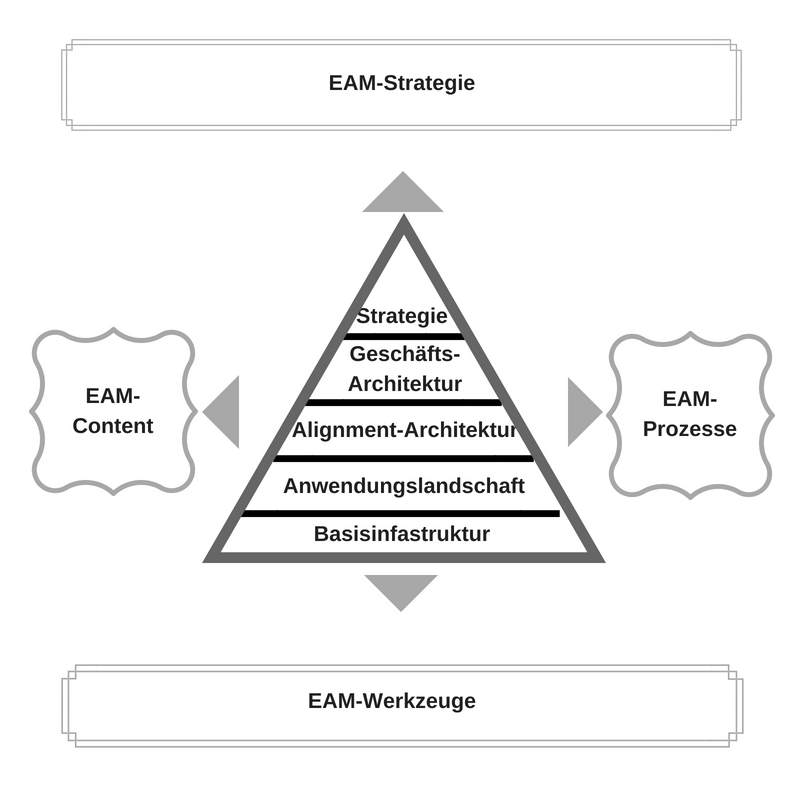
\includegraphics[width=0.75\textwidth]{Abbildungen/Pyramide.png}
\caption{EAM Pyramide und Handlungsfelder nach \textcite{Keuntje2010}}
\label{fig:pyramide}
\end{center}
\end{figure}

Die Organisation der EAM-Pyramide ermöglicht die gesamte Bandbreite der Geschäftsaktivitäten als Ganzes zu sehen. Dies erleichtert es dem EAM-Team, sich auf bestimmte Ziele konzentrieren und die Verfahren in der Reihe nach zu befolgen, damit sie nicht ihre Zeit mit anderen anstrengenden und zeitraubenden Projekten verlieren. Die vom Leser gesehene Klassifizierung der Ebenen gliedert sich in die 5 Unterstufen.

\paragraph{Strategie}
Auf der oberste Ebene wird die Unterstützung von Geschäftsmodellen durch technologische Leistengen gelingen, um eine zusammenhängende erfolgreiche Geschäftsstrategie zu erreichen, die die unteren Ebenen der Pyramide steuern kann.
\paragraph{Geschäftsarchitektur}
Auf dieser Ebene wird die gesamte Kultur der Organisation und die Besonderheit ihrer Funktion beschrieben (Standort, Leistungen, Produkte, Dienste, Organisation).Diese helfen bei der Entwicklung eines Architekturmodells und der Unterstützung der Bebauungsplanung.
\paragraph{Alignment-Architektur}
Die mittlere Ebene der Pyramide bildet die Verbindung zwischen den Geschäftsarchitektur und Anwendungslandschaft. An diesem Punkt wird der aktuelle Stand den Anwendungen mit den Geschäftsprozessen und Geschäftsfähigkeiten  neu justiert, damit die Geschäftsarchitektur auf die oberste Ebene anpassen kann.
\paragraph{Anwendungslandschaft}
Die Anwendungskomponente können über Dienste, Schnittstellen und IT-Werkzeuge die Anwendungen integrieren und nach fachlichen Punkten zu Anwendungsplattformen gruppieren.
\paragraph{Basisinfastruktur}
Auf der unteren Ebene befinden sich die IT Architekturelemente einer Firma. Hardwarekomponeneten (Netze,Speicherlösungen) und die Technologiekomponente (Betriebsysteme, Datenbanksysteme) werden durch Technologie Normen standardisieren und skalierbar zu gestalten.

Die Pyramide ist das Herzstück der Tätigkeit von EAM, aber um die Architektur wertschätzen zu können, müssen die Felder in Kontakt mit ihr bleiben. Jeder von ihnen trägt unterschiedlich zur Gründung von EAM bei und ist verantwortlich für verschiedene Arbeiten.

%%%

\paragraph{EAM Strategie}
Die EAM Strategie basiert auf der Festlegung von Zielen, Kosten, Nutzen und dem reibungslosen Ablauf von EAM. Als ersten Schritt im Integrationsprozess leiten die Architekten die Erstellung eines EAM-Teams, um den Fortschritt des Projekts zu überwachen und anzupassen und dann empfehlen sie die Bestimmung von 4 Paketen:
%%%%%%

\subparagraph{EAM Maturity Check}
Hier wurde die bereits vorhandenen Unternehmensarchitektur, die Art ihrer Verwaltung und die existierenden Elemente, der IT Manager helfen, die Unternehmenskultur zu verstehen und die Ist-Zustand zu bestimmen. Die Erstellung eines Fragebogens wäre sehr hilfreich.

\subparagraph{EAM Business Case}
Damit Unternehmer Kosten und Nutzen von EAM berechnen können, ist es wünschenswert ein Business Case, die die Nutzungspotenziale und Gewinne dieser Investition erfasst.

\subparagraph{EAM Ziele und Kennzahlen}
Die Festlegung von strategischen, taktischen und operativen Zielen ist es sehr wichtig um geschäftlichen Anforderungen auszurichten. Durch die Ziele den Nutzen werden einige wesentlichen Kennzahlen zum Messen der Ziellerreichung für EAM anzuordnen.

\subparagraph{EAM Programm und Roadmap}
An diesem Punkt wird die Formulierung des Einführungsplans gemacht. Also alle Regeln und Aktivitäten, die in den verbleibenden Handlungsfeldern und ihrer Synchronisation folgen werden.
%%%

\paragraph{EAM-Content}
Mit der Hilfe einem EAM-Werkzeug oder Framework wird ein geeignetes Metamodel entwickelt. Die Modellierungsprinzipien mussten deutlich die Richtlinien den Ebenen der EAM Pyramide betrachten und den Plan für Stufe vorsichtig entwerfen.

\paragraph{EAM-Prozesse}
Bei diesem Feld werden manche Schritte gemacht um die Unternehmensarchitektur mit strategische und taktische Planung, nachhaltig steuerbar zu machen. Lösungsszenarien werden entwickelt damit die Beteiligten herausfinden können mit welchen Anwendungen, die geschäftliche Anforderungen umgesetzt werden, um eine optimale Bebauung von Anwendungen zu erreichen (Bebauungsplan).  Nach der Beschaffung des Bebauungsplans folgt seine Übergabe im Bereich IT-Projekt-Portfolio Management damit die finanzielle Kontrolle und Durchführung des Projekts mit der notwendigen finanziellen Zuteilung des Plans verwirklichen kann.

\paragraph{EAM-Werkzeuge}
Die EAM-Tools zentralisieren die verteilte Dokumentation der Unternehmensarchitektur. Es gibt viele Arten von Werkzeugen, aber es ist sehr wichtig, das geeignete Werkzeug für die neue Architektur zu finden. Hier sollte Das Ist-Zustand berücksichtigt werden, damit Anwendungen mit EAM-Tools abgeglichen werden können. Der Schwierigkeitsgrad ist Heutzutage eine Entscheidung über einen modernen und nachhaltigen Werkzeug zu treffen.

Wie aus dem Zusammenhang ersichtlich ist, gibt es eine große Menge an Anpassungsmaßnahmen, die das Unternehmen in die verschiedenen Bereiche des Unternehmens integrieren muss. Viele Arbeitseinsätze müssen geändert werden, die Archive werden diversifiziert, der Alltag der Mitarbeiter wird sich ändern.

\section{Einflussfaktoren}
\subsection{Erfolgsfaktoren}
Es ist Zweifelhaft für das Unternehmen manchmal zu schauen ob EAM  einen Wertbeitrag erzeugt. Manche merken dass die Umsetzung fachlicher Anforderungen in Anwendungen länger dauert und teurer ist als zuvor ohne EAM.
Der Erfolg oder Misserfolg jedes Projekts wird nicht nur von direkten Teilnehmern, sondern auch von einer Reihe von externen Akteuren bestimmt. Er  liegt vor allem in einer Vielzahl kritischer unterschiedlicher Faktoren. \autocite{Bitkom2011}

\paragraph{Schnelle Ergebnisse}
Das Projekt muss das Erreichen kurzfristiger Ziele sicherstellen. Es ist wichtig, das Interesse des Managements am Projekt wach zu halten. Um dies zu erreichen, muss es schnell die notwendigen Ergebnisse für das Unternehmen erzielen. Wenn unmittelbare Ergebnisse nicht innerhalb von 3 Jahren auftreten, wird das Interesse am Projekt deutlich reduziert.
\paragraph{Top-Manager}
Sein Hauptzweck ist es, Probleme in der Organisation zu identifizieren und zu beseitigen. CIOs müssen nicht nur Probleme rechtzeitig identifizieren, sondern auch eine klare Vorstellung von den Ansätzen haben, die in jedem konkreten Fall anzuwenden sind.
\paragraph{Schrittweises Vorgehen zum Erreichen gesetzter, messbarer Zwischenziele entlang einer definierten Roadmap}
Das Top-Management soll die Richtlinie der Roadmap verfolgen und die Handlungsfelder für EAM Schritt für Schritt durchführen.
\paragraph{Taktisches Handeln entlang der Strategie}
Es ist sehr wahrscheinlich wegen der verschiedenen Ziele im Plan (Bugdet, externe Einflussfaktoren, Zwecke von EAM), dass Konflikte zwischen den Mitgliedern des EAM-Team entstehen. Für jede Lösung müssen Nutzen, Zeitpläne, Kosten und Risiken bewertet, und die Bebauungspläne berücksichtigt werden.
\paragraph{Begreifen der Unternehmensarchitektur als ein sich evolutionär weiterentwickelndes  Ganzes}
Manchmal läuft die Unternehmensarchitektur nicht so wie geplant, und es gibt zwischen dem Ist-Zustand und dem Soll Zustand einen Unterschied. Ein gute Praxis in einer solchen Situation wäre, wenn die entsprechenden Personen flexible auf diese Fälle reagieren können.
\paragraph{Kommunikation zwischen der IT-Organisation und der Business-Organisation mit den Geschäftsbereichen}
Es ist manchmal Zweifelhaft für das Unternehmen zu erkennen, ob EAM nützlich ist und einen Wertbeitrag liefert. Manche merken, dass die Umsetzung fachlicher Anforderungen in Anwendungen länger dauert und teurer ist als zuvor ohne EAM.
\paragraph{Kommunikation innerhalb der IT-Organisation}
Die Unternehmensarchitekten , die für zugewiesene Geschäfts- und IT-Domänen das Know-How für die Projekte bereitstellen, sollten die Kommunikation mit dem zentralen EAM-Team vermittelnd betreiben, damit die Projekte richtig durchgeführt werden \autocite{Korotkov2013}.

Die einzelnen Verfahren müssen auf der Grundlage des vorbereitenden Plans durchgeführt werden. Der Manager sollte umgehend auf individuelle Änderungen reagieren und das Team koordinieren, so dass Probleme in der Übergangsphase des Projekts vermieden werden können. Die besten Strategien scheitern nicht, weil sie nicht wachsen können, sondern weil es sehr schwierig ist sie zu bedienen. Die Aussichten sind in der Regel nicht durch das Managementsystem selbst beschränkt, sondern durch die wirtschaftliche Realität. % Daher ist das Hauptziel der erfolgreichen Verwaltung der Konfigurationsmanager der Wunsch nach Selbstverbesserung und Bedingungen für die Schaffung einer kohärenten Gruppe und geistiger Entwicklung ihrer Mitglieder zu schaffen.

Daher sollte eine effiziente Architektur diese oben genannten Trends harmonisch kombinieren. Die Verwendung aller aufgeführten Funktionen führt zu dem gewünschten Ergebnis und hilft, die dem Manager zugewiesenen Probleme und Aufgaben zu lösen. Ein moderner Manager sollte in der Lage sein, das Problem aus verschiedenen Blickwinkeln zu sehen und eine ausgewogene, vielschichtige und ganzheitliche Sicht auf alle zu haben, als auch sich zu entwickeln und ihre persönliche Effektivität zu steigern. Die Verwendung von allen registrierten Kompetenzen durch den Treuhänder wird das gewünschte Ergebnis so schnell wie möglich geben und die Probleme und Aufgaben an den Administrator delegieren.

\subsection{Misserfolgsfaktoren}
All dies wird sehr optimistisch beschrieben. Es kann sehr leicht sein, den Fehler zu machen und gegen einige Regeln zu stimmen und die Vorschriften nicht zu berücksichtigen. Der Manager sollte nicht nur die Erfolgsfaktoren kennen, sondern auch die Faktoren des Scheiterns betrachten.
%Es ist sehr nützlich, um die ineinandergreifenden Menschen zu wissen, welche Maßnahmen sollten Sie vermeiden, bevor Sie schnell reagieren kann, wenn Sie feststellen, dass ein Dienst, der ‚eine Entscheidung, die Leitungen genommen wurde das Projekt zu kollabieren.
Jüngsten Berichten zufolge \textcolor{red}{(Quelle?)} scheitern 66\% der IT-architektonischen Geschäftsinitiativen. Aber warum? In den letzten Jahren gab es viele Diskussionen, Expertenmeinungen und schriftliche Stellungnahmen zu diesem Thema.
Die Geschäftsarchitektur wurde vor ein paar Jahren entwickelt, um der wachsenden Komplexität von IT-Systemen und ihrer schlechten Ausrichtung auf Geschäftsziele gerecht zu werden. Dieselben Probleme bestehen auch heute noch und werden durch den beschleunigten technologischen Wandel verstärkt.
Im Folgenden finden Sie eine Liste, warum viele Enterprise Architecture-Initiativen fehlschlagen \autocite{Kabai2010}:


\paragraph{Der falsche Lead-Architekt}
Eine Person kann EA verstehen, hat jedoch ineffiziente Führungsqualitäten, die nicht zu einer guten Organisationsstruktur und Personalstärke beitragen können.
\paragraph{Überwachung und Inflexibilität gegenüber der Unternehmenskultur}
Für eine erfolgreiche EA muss die Unternehmenskultur bei der Planung und Gestaltung von EA für die Organisation berücksichtigt werden.
\paragraph{Verspätete Einführung einer effektiven EA-Governance}
EA-Governance-Prozesse müssen so früh wie möglich festgelegt werden, statt auf mehr Architekturinhalte zu warten.
\paragraph{Nicht genug Zeit für Kommunikation}
Unternehmensarchitekten müssen die Mitarbeiter unterrichten. Es ist effizient, dass Organisationen einen EA-Kommunikationsplan mit Nachrichten entwickeln und ausführen, die auf jede Zielgruppe zugeschnitten sind.
\paragraph{Die Auswirkungen nicht messen und nicht kommunizieren}
Der Wert von EA ist oft indirekt, was das EA-Programm dem Risiko des Scheiterns aussetzt. Es wird empfohlen, dass Unternehmensarchitekten eine Präsentation geben, um jede Erfolgsgeschichte von EA, die auf ein Projekt angewendet wird, zu demonstrieren.
\paragraph{Nicht nur Technical Domain-Level-Architektur}
EA ist viel breiter, sie umfasst Business-, Informations- und Lösungsarchitektur und nicht nur die technische Domäne \mbox{\autocite{Ojo2016}.}
\paragraph{Mangel an Sponsoring}
Gut gesponserte Architekten können Vertrauen aufbauen, indem sie konsistent aussagekräftige Ergebnisse liefern. Ein Mangel an Sponsoring wird sogar die besten Architekten zum Scheitern bringen.
\paragraph{Wartung der EA Artifact Factory}
EAM-Teams sollten sich darauf konzentrieren, häufige, aussagekräftige und messbare Geschäftsergebnisse zu erzielen.
\paragraph{An ein bestimmtes Framework oder einem Tool klammern}
Es gibt mehr als 80 EA-Frameworks. Der beste Ansatz besteht darin, alle wichtigen Frameworks zu kennen, das meiste von dem, was Sie gelernt haben, zu verwerfen und die verbleibenden 10\% auf eine Weise zu mischen, die der Unternehmenskultur, der Reife und den Geschäftszielen entspricht.
\paragraph{Denken, dass Enterprise Architecture der Technologiearchitektur entspricht}
Die meisten EA-Programme werden von der IT initiiert und kommen nie über den Technologiebereich hinaus. Obwohl Technologiestandards, Technologie-Roadmaps und solide technische Verfahren einfachere, billigere, tragbare, wiederverwendbare und besser unterstützte Lösungen bieten, stimmen sie Ihre IT-Investitionen nicht mit den Geschäftszielen ab und werden Ihr Unternehmen nicht mit technologischen Innovationen versorgen.
\paragraph{Das Wort Enterprise wörtlich nehmen}
Um IT-Architektur auf die reale Unternehmensebene zu bringen, bedarf es einer ausgereiften und engagierten Organisation. Wenn man versucht, den Unternehmensaspekt zu früh zu weit zu schieben, wird man scheitern.

Die erfolglose Umsetzung von Entscheidungen, ihre unnötige Arbeit oder Inkongruenz mit den am Arbeitsplatz gesetzten Zielen wirkt sich unmittelbar auf andere Ebenen aus. Beispielsweise kann eine falsch entworfene Anwendung die organisatorische Leistung beeinträchtigen. Dies wiederum kann den Gewinn aus den Dienstleistungen für die Kunden reduzieren.
Das Problem wird durch die Tatsache verstärkt, dass diese negativen Effekte schwer zu bestimmen sind, wenn die Messung der Erfolgskriterien nur schlecht oder nicht koordiniert zwischen den Ebenen erfolgt.

Jede Veränderung in einem Geschäft wie im täglichen Leben des Menschen folgt einer Vielzahl von Entscheidungen, die wir treffen.
Um also die Architektur des Unternehmens erfolgreich zu verändern, müssen wir berücksichtigen, was genau geändert werden muss, wann es geändert werden muss und wen es ändern wird.
Das Erzielen einer effizienten EAM ist eines der wichtigsten Geschäftsziele. Viele Unternehmen haben von seiner Konsolidierung profitiert. %Wie weiter erhöht den Bedarf an den technischen Fortschritt und die Entwicklung neuer Anwendungen, Programme, fühlen sich mehr Unternehmen Systeme, die die Voraussetzung für die Gestaltung einer solchen Architektur. //
Im Anschluss an den technologischen Fortschritt ist es selbstverständlich, dass nicht nur der private Sektor oder ein bestimmtes Unternehmen in einer Wirtschaft schrittweise entwickelt wird. Der Fortschritt eines Landes hängt auch von der Regierung, ihrem Bildungssystem und ihrem gesunden Bankensystem ab.
% Jiota ist nervös. OK. MAU MAU MAU MAU. KRAULITZA MAU MAU MAU MKRAUUUUUUUU KRAUUUUUU KRAUUUUUUU UUUUUU UUU LIIIII UAAAZZAAAAA.
Um diesen technologischen Fortschritt in einem Land zu erlangen und transparent zu halten als auch die Bürokratie zu reduzieren (etwas, das viele Länder wünschen), sollten andere Wirtschaftsbereiche mit einer technologischen Architektur ausgestattet werden.

\section{Fallbeispiele}
In diesem Kapitel werden die Vorteile des EAM in verschiedenen Sektoren betrachtet. Für Banken folgen Beispiele zum sog. BIAN, für Regierungs-EA von Dänemark und den Niederlanden und dem Experiment von Norwegen für die Einrichtung von EA für Universitäten.

\subsection{EA im Bankensektor}
\subsubsection{EAM Banken}
Der Markt ist in den letzten Jahren gleich geblieben, aber der Wettbewerb ist zu stark gestiegen. Hier ist es für eine Bank wichtig, ihre bestehenden Kunden und Neukunden, insbesondere junge Menschen, mit interessanten neuen Produkten, Dienstleistungen und Technologien zu erreichen, die auf eine langfristige Kundenbindung an das Unternehmen abzielen.

Die Banken müssen zahlreiche regulatorische Maßnahmen einhalten und auf die rasche Umsetzung neuer Geschäftsanforderungen, gestiegene Kosten und eine steigende Anzahl innovativer Produkte, die sich auf dem Markt befinden, reagieren. Es gibt einen anhaltenden Wettbewerb zwischen Banken und Newcomern und großen diversifizierten Unternehmen wie Facebook, eBay, Allianz, BMW oder Deutsche Telekom. Sie intervenieren in verschiedenen traditionellen Geschäftsbereichen, wie z Investitionstätigkeit, Zahlungsverkehr und die Vermögenswerte einer Bank und stoßen damit die traditionellen Kunden der Bank ab.

Um allen Kundengruppen gerecht zu werden, müssen unterschiedliche Vertriebskanäle angeboten werden. Viele Kunden nutzen Mobil oder Online-Dienstleistugen. Sie können unterschiedliche Verfahren entweder mit der Hilfe eines Bankberaters oder eines Filialmitarbeiters anwenden.
Andere Kunden bevorzugen den  Selbstbedienung--Bereich einer Bank  zu nutzen, um ihre Transaktionen durchzuführen, Überweisungen zu machen und Kontostände zu kontrollieren. 

Die Geschäftsarchitektur der Bank kann helfen, verschiedene Bankverwaltungssysteme aufzubauen und die Arbeit der Abteilungen und Geschäftsprozesse der Bank zu organisieren und zu verbessern. Bis heute reichte das effiziente Management der Ressourcen und Operationen der Banken nicht aus, um stabiles Wachstum und Wettbewerbsvorteile zu erzielen. Die Banken müssen auf ein neues Niveau, um Wachstum und kontinuierliche Verbesserung zu erzielen. \autocite{Kamarianakis2016}

Kundenanforderungen müssen wahrgenommen werden und die Verfügbarkeit neuer Apps wachsen. Worauf man sich jedoch konzentrieren sollte, sind die Vorteile, die sich aus diesem ständigen Veränderungsdruck ergeben. Im Folgenden sind einige der Vorteile aufgeführt, die die Banken und ihre Mitarbeiter durch die Anwendung einer solchen Architektur erzielen können:

\begin{APAitemize}
\item Verbesserte Erfahrung und Produktivität des Arbeitgebers 
\item Konsequentes, beeindruckendes, über die Bank hinweg integriertes Kundenerlebnis
\item Effektive Funktionen zur Steigerung der Produktivität und des Kundenservices
\item Reduzierung des operativen Risikos
\item Technologie, die flexibel, zuverlässig und immer verfügbar ist
\item Standardisierte Technologieplattformen
\item Infrastruktur, die sicher und geschützt ist
\item Reduzierung und Vereinfachung der betrieblichen Systeme
\end{APAitemize}

\mbox{}

Eine Bank möchte das bestehende Kundenmanagementsystem verbessern. Um eine Entscheidung für einen Kunden zu treffen, der beispielsweise einen Kredit erhalten möchte. Die Bank sollte alle Daten des Kunden sammeln, sie überprüfen und einige Daten mit vorherigen statistischen Erhebungen vergleichen, um ein Angebot bieten zu können.

Daher beschrieb das IT-Team in einer kurzen Zusammenfassung die geschäftlichen Vorteile des neuen Architekturdesigns. Anhand einer einfachen Grafik davor und danach zeigte das Team, wie eine fragmentierte Architektur mit vielen verschiedenen Zahlungssystemen in eine stärker integrierte, grenzüberschreitende IT-Umgebung rationalisiert werden kann.

\begin{figure}[!htbp]
\begin{center}
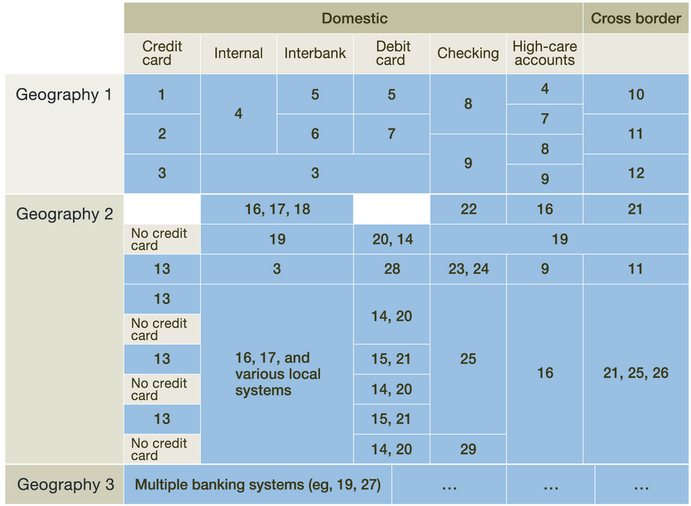
\includegraphics[width=0.75\textwidth]{Abbildungen/McKinsey1.png}
\caption{IT-Landschaft vor EAM \autocite{McKinsey}}
\label{fig:McKinsey1}
\end{center}
\end{figure}



\autoref{fig:McKinsey1} zeigt die Umstrukturierung der inländischen, regionalen und grenzüberschreitenden Transaktionen einer Bank. Was beobachtet wird, ist eine fragmentierte Architektur mit vielen verschiedenen Zahlungssystemen und vielen verstreuten Anwendungen. Akquisitionen, interne Expansion und eine Reihe neuer Produkte hat für die Bank über die Jahre ein Netzwerk von schlecht vernetzten und redundanten System hervorgebracht.

%\newpage

\begin{figure}[!htbp]
\begin{center}
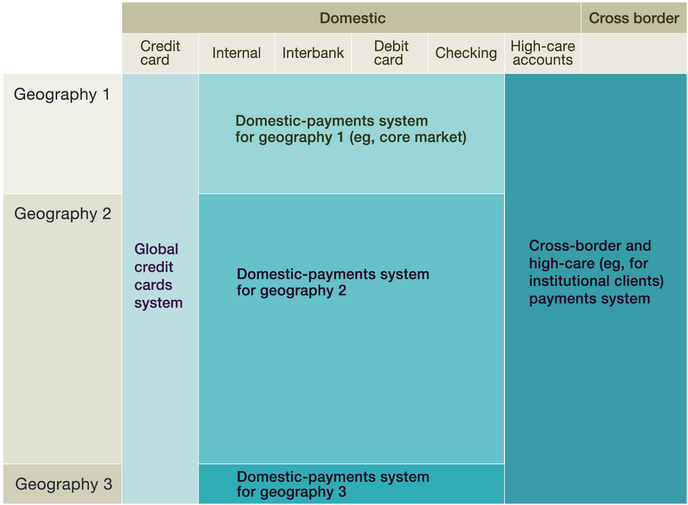
\includegraphics[width=0.75\textwidth]{Abbildungen/McKinsey2.png}
\caption{IT-Landschaft nach EAM \autocite{McKinsey}}
\label{fig:McKinsey2}
\end{center}
\end{figure}

Nach Implementierung von EAM (\autoref{fig:McKinsey2}) werden durch die neue Architektur der Bank die regionalen Lösungsansätze für Inlandszahlungen und die globalen Lösungsansätze für Kreditkarten als auch grenzüberschreitende Transaktionen weniger, und  stattdessen werden mehr integrierte Anwendungssysteme eingesetzt.

\subsubsection{BIAN}

Die ganze Welt erlebt jetzt eine Phase der Innovation. Großes Interesse wurde von der internationalen Vereinigung BIAN (Banking Industry Network Architecture) erworben worden, deren Mitglieder die führenden Architekten der Banken (ABN AMRO Group, Société Générale Gruppe, Unicredit Group, etc.), Anbieter von Bankensoftware und Service-Provider (IBM, SAP, Microsoft und andere). Diese Modell repräsentiert Logik, Wissen und Design von Service-Sektor-Metadaten, die durch das Banking Framework definiert werden.
 
Laut Gartner Group Inc. bevorzugen heute 80\% der Banken, dass sich ihre IT-Strategien auf SOA oder zumindest auf ein hybrides (serviceorientiertes) Architekturmodell anzupassen. Das Netzwerk wurde im April 2008 als unabhängige Non-Profit-Organisation gegründet, um die IT-Standards für Bankinteroperabilitätsdienste zu definieren.

Das BIAN-Framework wurde entwickelt, um Geschäftsszenarien in einer Vielzahl von Arten von Institutionen zu unterstützen. Viele Finanzinstitute wollen das BIAN-Framework nicht in einem grünen Feld implementieren, sondern wollen ihre Architektur in Übereinstimmung mit BIAN transformieren. BIAN ist ein Joint Venture von Stakeholdern,  BIAN Manager, Architektur Group, Finanzinstitute, Softwareanbieter und Beratungsunternehmen, die im Laufe des Jahres in Kongresse zusammentreffen. BIAN hat nur eine Art von Mitgliedschaft, die allen Mitgliedern die gleiche Stimme und Macht verleiht. Der jährliche Mitgliedsbeitrag von BIAN beträgt ca. US\$\,30.000.

Die Verwendung eines standardisierten Frameworks wie BIAN kann dazu beitragen, die Komplexität Ihrer Infrastruktur zu reduzieren, indem Sie die Architektur, Prozesse und Kanäle der Bank strukturieren und strukturieren. Es wird eine Reihe von Diensten und Metadaten eingeführt, die es Organisationen ermöglichen, Kundeninteraktionen zu optimieren, die Datenqualität zu erhöhen und doppelte Systeme und Daten zu reduzieren. \autocite{BIAN}

Die Registrierungskosten sind hoch und die Installation teuer, aber es lohnt sich, einen solchen Framework zu schaffen, da sich die Organisation mit ihrer Einführung dynamisch ändern wird. Mit den BIAN SOA-Framework erhalten Kunden Zugang zu den mit diesem Serviceangebot in Zusammenhang stehenden Daten in Echtzeit, als auch erzielen  gleichzeitig Markt- und Kosteneinsparungen.

Es gibt viele Gründe, warum die Übernahme des BIAN-Frameworks an Dynamik gewinnt. Die Vorteile der Verwendung sind unten angegeben \autocite{BIAN2}: 
\paragraph{Reduziert die Komplexität}
Die Bank-Architektur basierte bisher auf alter Infrastruktur und es ist schwierig, dieses komplexe Netzwerk von Systemen mit neuen Technologien zu integrieren, wie Web, Mobile und BPM. Angesichts der zahlreichen Fusionen und Übernahmen, die der Bankensektor Anfang der 2000er erlebte, ist eine weitere Modernisierung des Bankensektors erforderlich.
\paragraph{Reduktion von dualen Systemen}
Die Existenz mehrerer Dateisysteme, Datenbanken, Content-Repositories, Lieferanten, Anwendungen und Tabellen macht die Ausführung von Verfahren umständlich und behindert die Qualität der Dienstleistungen. Die Anwendung des Frameworks erhöht die Gültigkeit den Daten.
\paragraph{Kostenreduzierung}
Durch die Nutzung des BIAN-Frameworks zur Transformation des Unternehmens werden die Struktur des Unternehmens geformt und im Laufe der Zeit die Kosten reduziert.
\paragraph{Interoperabilität}	
BIAN-Dienste sind modular aufgebaut und können je nach Unternehmensanforderungen intern, in einer privaten Cloud oder in einer öffentlichen Cloud gehostet werden.
\paragraph{Sicherheit}
Datenbezogene Sicherheit wird aufgrund der Konzentration von Daten und der Standardisierung von SOA-Schnittstellen und der Verringerung der Anzahl von Datenübertragungen zunehmen.
\paragraph{Outsourcing von Dienstleistungen}
Neue serviceorientierte Partner werden damit beginnen, Angebote zu entwickeln, die es ermöglichen, dass Teile Ihrer Referenzarchitektur entweder in Cloud gehostet oder sogar ausgelagert werden. Die Partner werden ihre Angebote als BIAN-kompatibel gestalten. Beispiele hierfür sind: Kreditprüfungsdienste, 
Kreditgeberlösungen, Enterprise Content Management (ECM), Kundencenter für Telefon, E-Mail, SMS usw.

\subsection{EA in Regierungen}
\subsubsection{EA in Regierungen}
Immer mehr Länder versuchen, das Steuersystem durch nationale eGovernment-Strategien und mehrjährige Aktionspläne zu ändern. EA ist ein effektives strategisches Planungsinstrument, um  einfacher Verbindungen zu schaffen und die Interoperabilität zwischen den Regierungen zu verbessern \autocite{Bakar2016}. Regierungen in verschiedenen Ländern versuchen, ihre Systeme zu verbessern und Bürokratie abzubauen. Das Problem in diesem Fall ist, dass jedes Land andere Wachstumsraten und andere Informationssysteme hat. Die Technologiekarte unterscheidet sich daher von Land zu Land. Haiyan Qian, Direktor der Abteilung für Öffentliche Verwaltung und Entwicklung, Abteilung der Vereinten Nationen Wirtschaft und Soziales (UNDESA) :
\begin{quote}
\glqq EA ist ein effektives strategisches Planungsinstrument für indem die Schaffung von Verbindungen erleichtert und die Interoperabilität zwischen den Regierungen verbessert wird Regierungsstellen, die sowohl internen Geschäftsprozessen als auch verbesserten Geschäftsprozessen zugute kommen Bereitstellung öffentlicher Dienstleistungen für die Bürger.\grqq
\autocite{Pallab2010}
% Quelle Haiyan Qian
\end{quote}
Es gibt wenige Male, in denen einige Staaten versucht haben, ihren öffentlichen Sektor zu transformieren und einen integrierten Ansatz für die Strategie der öffentlichen Architektur zu erreichen.


\begin{table}[!htbp]
\caption{Vorteile von EA in Regierungen \autocite{Pallab2010}}
\begin{center}
\begin{tabularx}{\textwidth}{|X|X|}
\hline
Intern & Extern \\
(An Provideragenturen und Regierungen) & (An Verbraucher und Unternehmen \\\hline
(1) Vermeidung von Doppelarbeit				& (1) Schnellere Service-Lieferung \\
(2) Reduzierung der Transaktionskosten		& (2) Größere Wirksamkeit \\
(3) Vereinfachte bürokratische Verfahren	& (3) Erhöhte Flexibilität der Service-Nutzung \\
(4) Mehr Effizienz							& (4) Innovation in der Dienstleistungserbringung \\
(5) Reichere Kommunikation und Koordination	& (5) Mehr Beteiligung und Einbeziehung \\
(6) Verbesserte Transparenz					& (6) Mehr Bürgernähe \\
(7) Mehr Informationsaustausch				& (7) Größere Offenheit und Transparenz \\
(8) Sichere Informationsverwaltung			& \\\hline
\end{tabularx}
\end{center}
\label{tab:InternExtern}
\end{table}

Die Vorteile eines solchen Modells (\autoref{tab:InternExtern}) sind in  nicht nur von der Seite den öffentlichen Hand (Links) sondern auch von der Seite den Unternehmen. Die Vereinigte Städte sind überzeugt, dass  Dienste mit Informationstechnologie (E-Service) können tatsächlich das Tempo und die Qualität der öffentlichen Dienstleistungen in Zeiten der Wirtschaftskrise verbessern. Folglich sind die Regierungen, die mit den Informationstechnologien verbunden sind, ein Schlüsselelement für eine gesunde Ökonomie.

Der Literatur zufolge wurden verschiedene Konsolidierungen in jedem Land verwendet, um das Ziel zu erreichen, weil jeder Staat  sein eigenes Temperament und seine eigene Struktur hat. Das folgende Diagramm veranschaulicht alle Integrationsphasen, die im Laufe der Zeit für die verschiedenen Regierungen formuliert wurden, die versucht haben, EA umzusetzen. Die Transformation der Regierung ist eine langfristige Anstrengung, die von vielen Faktoren beeinflusst wird. Der Übergang zu einer technisch einheitlichen Regierung erfordert die Implementierung aller Phasen der E-Government Fähigkeit und Reife, jeder repräsentiert eine progressiv höhere Ebene bei der Umwandlung der Regierung.

Mit der Hilfe der \autoref{tab:PhasenModelle} ist es leicht zu erkennen, dass jedes Jahr neue Modelle entwickelt wurden, die versucht haben, zur EA-Integration beizutragen und die vorherigen Phasen der neuesten Modelle zu verbessern.

\begin{table}[!htbp]
\caption{Phasen-Modelle aus \textcite{Napitupulu2016}}
\begin{center}
\begin{tabularx}{\textwidth}{|X|X|}
\hline
Modell & Phasen \\\hline
Gartner's Vier-Phasen-Modell 2000
&
(1) Web Präsenz,
(2) Interaktion,
(3) Transaktion,
(4) Transformation
\\\hline
UNS' Fünf-Phasen 2001
&
(1) Entstehenden,
(2) Verbessert,
(3) Interaktiv,
(4) Transaktional,
(5) Integriert
\\\hline
Deloitte und Touche's Sechs-Phasen-Modell 2001
&
(1) Informationspublishing / Verbreitung,
(2) Offizielle Zwei-Wege-Transaktion,
(3) Mehrzweck-Portale,
(4) Portalpersonalisierung,
(5) Clustering von gemeinsamen Diensten,
(6) vollständige Integration und Enterprise-Transaktion
\\\hline
Hiller und Belanger's 2001 und Moon's 2002 Fünf-Phasen-Modell
&
(1) Einfache Informationsverarbeitung,
(2) Anfrage und Antwort,
(3) Service und finanzielle Transaktion,
(4) Vertikale und horizontale Integration,
(5) Politische Beteiligung
\\\hline
Siau und Yong's Fünf-Ohasen Synthetisiertes Modell 2005
&
(1) Web-Präsenz,
(2) Interaktion,
(3) Transaktion,
(4) Transformation,
(5) e-Demokratie
\\\hline
\end{tabularx}
\end{center}
\label{tab:PhasenModelle}
\end{table}

Aufgrund der Vielfalt der nationalen, die technologischen Infrastrukturen, der Institutionen und der Ziele des Staates, alle Entwurfs- und Umsetzungsmodelle von EA könnten nicht die gleichen Auswirkungen haben. Der nächste Abschnitt beschreibt, wie zwei Länder versuchen, einen gemeinsamen Rahmen zu schaffen.

\subsubsection{NEA (NL, DK)}
Als ein Beispiel für die Regierungsarchitektur werden im Text die Bemühungen zweier europäischer Länder zur Gründung von EA analysieren. \autocite{Janssen2007} Die beiden Nationen der Europäischen Union sind Dänemark und die Niederlande, und ihr Architekturplan heißt NEA (National Enterprise Architecture). Die schrittweise Umsetzung der NEA würde auf die folgenden Schritte zurückgeführt.

Die Entscheidung, eine NEA zu treffen, wird von der politischen Governance beschlossen und findet unter Verwendung verschiedener Governance-Mechanismen statt. Der Architekt untersucht die Ressourcen der öffentlichen Meinung, den Implementierungsrahmen und die Methoden des Planungsprozesses, um die Reformen aufzeichnen zu können. Der Architekt verwendet dann Leitlinien, um das Projekt zu führen. Das Erreichen des Projekts wird durch die Koordination vieler Organisationen und wissenschaftlicher Disziplinen erreicht.

Hier ist es sehr wichtig, auf die Wahl dieser Länder zu verweisen. Es sollte verstanden werden, unter welchen Kriterien die Länder eine solche Strategie gewählt haben und wieso sie ein Vergleichsmaßstab sind.
Beide Länder:
\begin{APAitemize}
\item haben eine ähnliche politische und institutionelle Struktur
\item haben ein kapitalistisches System und parlamentarische Republiken
\item befinden sich hinsichtlich der Forschungsreife in den ersten zehn Ländern
\item genießen ein hohes Maß an Autonomie bei ihren eigenen Entscheidungen
\item haben ihre finanzielle Kontrolle und können unabhängig Investions-Entscheidungen treffen
\item sind hierarchisch organisiert und haben eine autonome Koordination
\end{APAitemize}
Dänemark hat den Entwurf der NEA sehr früh dynamisch begonnen, aber dagegen die Niederlande einen vorsichtigen Stand haben, um Fehler und Risiken zu vermeiden. Dänemark hatte auch eine bessere Zusammenarbeit innerhalb der Regierungsebenen, während die Niederlande eine bessere Verwaltungsstruktur hatten, indem sie Ressourcenkontrolle und Portfoliomanagement verwendeten.

Trotz dieser Ähnlichkeiten haben diese Länder auch Ungleichheiten. Dänemark ist ein kleines Land mit 5,5 Millionen Einwohnern, während die Niederlande 16,3 Millionen Einwohner haben. In \autoref{tab:DKvsNL} sind alle Demografien aufgeführt, die 2005 gesammelt wurden, um einen neuen Plan zu erstellen.
% Quelle
\begin{table}[htbp]
\caption{Vergleich der IT-Landschaft zwischen Dänemark und den Niederlanden \mbox{\autocite{Janssen2007}}}
\begin{center}
\begin{tabularx}{\textwidth}{|X|c|c|}
\hline
& Dänemark & Niederlande \\\hline
Bürger (Millionen) & 5,41 & 16,34 \\\hline
Bruttoinlandsausgaben für F\&E (GERD) (\%) des BIP & 124,3 & 123,3 \\\hline
Arbeitslosenquote der Erwerbspersonen (\%) & 4,8 & 4,7 \\\hline
Ausgaben für öffentliche Verwaltung (\% des BIP) & 53,2 & 45,7 \\\hline
BIP Pro-Kopf-Kaufkraftstandard (KKS) (EU-25 = 100) & 2,56 & 1,76 \\\hline
Anzahl der Beamten (FTE) & 845.000 & 400.000 \\\hline
Mitarbeiter der Zentralregierung (FTE) & 80.000 & 120.000 \\\hline
Anzahl der Ministerien & 19 & 13 \\\hline
Jährliches IT-Budget (Milliarden \euro) & 0,8 & 2,3 \\\hline
Anzahl der Online-Dienste im Oktober 2004 (\%) & 82 & 70 \\\hline
Haushalte mit Internetanschluss  (\%) & 83 & 90 \\\hline
Haushalte mit Breitbandanschluss  (\%) & 40 & 50 \\\hline
\end{tabularx}
\end{center}
\label{tab:DKvsNL}
\end{table}
Für das E-Government-Projekt wurden demografische Merkmale untersucht und 18 Interviews mit Regierungsvertretern und Mitgliedern, die sich mit Geschäftsarchitektur befassen, durchgeführt

Laut den Interviews in den beiden Ländern wurde klar, dass die Gestaltung des NEA komplex ist und es ist die Teilnahme von vielen öffentlichen Einrichtungen und Institutionen abhängt. Öffentliche Dienste sind nicht immer in der Lage, alle Änderungen zu übernehmen und die Autonomie der Öffentlichkeit verhindert die Entscheidungsfindung. Die Ziele und Erwartungen der Befragten waren in jedem Land unterschiedlich. Das Ziel der dänischen Regierung war die Interoperabilität zu gewährleisten, aber das Ziel der niederländischen Regierung war Bürokratie zu reduzieren.

Beide Länder haben eine andere Verwendungsrichtung für NEA, aber beide verwenden jedoch ein Framework, das auf dem Zachman Model und auf SOA-Diensten basiert. Dieses Framework wird verwendet, um die Prinzipien der Architektur zu etablieren, um eine best practice zu ermöglichen. In \autoref{fig:EAMRegierungen} ist die Abbildung von dem Framework den Niederlanden gezeigt.
% Abbildung

\begin{figure}[!htbp]
\begin{center}
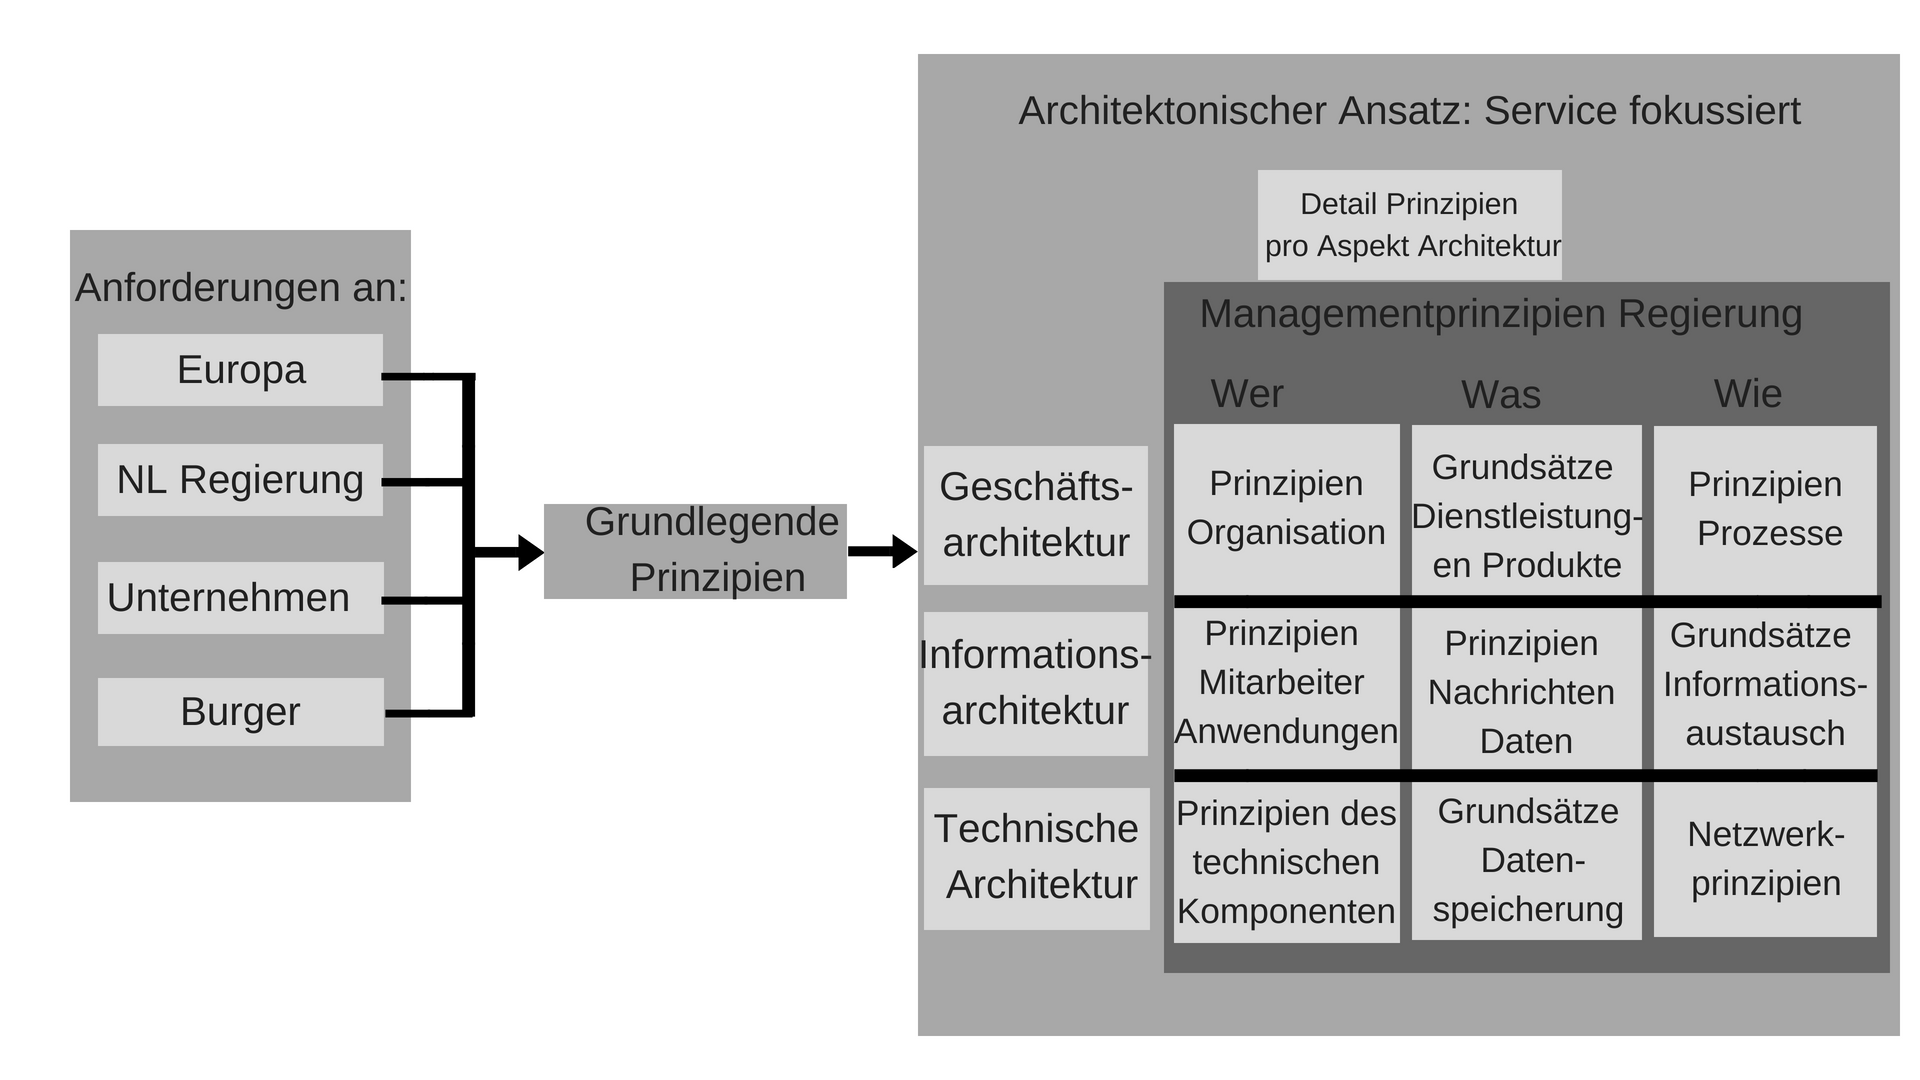
\includegraphics[width=0.75\textwidth]{Abbildungen/EAMRegierungen.png}
\caption{NEA Framework nach \textcite{Janssen2007}}
\label{fig:EAMRegierungen}
\end{center}
\end{figure}

\newpage
Die Annahmen von NEA basieren auf Freiwilligenarbeit und der Vision politischer Führer. Es gibt keine finanziellen Anreize und die Integration basiert auf der Notwendigkeit der Interoperabilität.

Mit diesem Framework kann die Komplexität von Systemen durch Vereinfachung der Arbeitsteilung der Beteiligten (Wer, Wo), Informationen (Was) und Infrastruktur (Wie) bewältigt werden. Die Strukturen im Regierungsrahmen unterscheiden sich stark von dem des privaten Sektors.

Die Befragten haben angegeben, dass das Zachman-Framework kompliziert und zu abstrakt sei, um die bestehenden architektonischen Probleme lösen zu können. Es wurde auch berichtet, dass die Behörden, die für dieEntwicklung von Regeln zuständig sind, keinen direkten Bezug zum EA-Programm haben.
% Quelle Zachmann-Modell

Im Allgemeinen wird der Eindruck erweckt, dass diese Strategie richtig ist, um Homogenität zwischen den Gemeinden  sicherzustellen, aber die Bestrebungen der politischen Führer waren erfolglos.
Beide Länder haben ihre Strukturen anders angepasst, um die Anwendung der NEA zu erreichen. Der Unterschied besteht darin, dass die dänischen Bemühungen  sich auf einzelnen Planungsprozesse konzentriert haben, während die niederländische NEA eine Reihe von Grundsätzen und Richtlinien befolgten, gemäß des Zachman-Modells.
% Quelle Zachmann-Modell

Dänemark kann viel von dem niederländischen Ansatz zum Anwenden bewährter Praktiken im NEA-Programm und seinem starken Fokus auf Bürokratieabbau lernen. Die Niederlande können von den Interoperabilitätskomponenten lernen und der Planungsprozess konzentriert sich auf die dänische NEA.
	
\subsection{EA im Bildungssektor}
\subsubsection{EA im Bildungssektor}
Die Einführung einer neuen Architektur in einer Organisation ist eine Herausforderung für den Bereich der Informatik. Es gibt Vorbehalte, wenn es um Bemühungen geht, eine neue Informationstechnologie in öffentlichen Institutionen zu implementieren.  die Einführung  von EA in nationalen Regierungen ist -  folgend den Ergebnissen des vorhergehenden Kapitels - schon schwierig, noch schwieriger gestaltet sich die Anwendung von EA an öffentlichen Universitäten und Hochschulen.	

Der Beitrag des EAs zum Bildungssystem ist ein Vorläufer der Regierungschefs, die eine Vision haben, das Bildungssystem ihres Landes zu verbessern und es dem Ministerium für Bildung zu ermöglichen, leichtere Entscheidungen zu treffen. \autocite{RSN2014}

Neben dem Ministerium werden die Bürger des Landes sowie andere Bildungsbereiche profitieren.
Im Folgenden werden die Vorteile für die Parteien näher erläutert \autocite{ICT2015}:
\paragraph{Studenten}
Sie werden in der Lage sein, den Unterricht leichter zu wählen, und es wird einfacher, den Studenten an eine andere Universität zu vermitteln. Fernunterricht kann erleichtert werden, und die Zuordnung der Kurse zwischen den Einrichtungen erfolgt automatisch.
\paragraph{Lehrpersonal}
Es wird eine erfolgreiche Durchführung von Vorlesungen durch Technologiestrukturen in Echtzeit möglich sein, wenn die Lehrer für eine Weile in anderen Ländern fehlen sollten. Die Auswertung der Ergebnisse der schriftlichen Tests könnte schneller erfolgen und es gäbe einen besseren Zugang zu den Unterrichtsmaterialien.
\paragraph{Forscher}
 Mit der neuen Architektur wäre ein einfacher Zugriff auf die Daten- und Qualitätsbewertung möglich. Forscher hätten die Möglichkeit, im Ausland zu arbeiten und von anderen Ländern finanzierte Umfragen durchzuführen
\paragraph{Management}
Durch Zusammenarbeit und Wissensaustausch würden neue wegweisende Ideen geboren. Eine Verbesserung der Qualität der Entscheidungsfindung würde durch die Verbesserung der Managementinformationen ermöglicht und die Komplexität der Verfahren würde verringert.
Verwaltungspersonal und IT-Abteilungen
Die Arbeitsteilung zwischen den verschiedenen Sektoren wäre institutionalisiert. Und die Mitarbeiter hätten eine bedeutende Erfahrung darin, einen solchen technologischen Wandel umzusetzen und ihren Lebenslauf zu bereichern.

Studierende profitieren von mehr Mobilität und Flexibilität bei der Anpassung des persönlichen Lernprozesses. Lehrende bieten bessere Möglichkeiten für Spezialisierung und vertiefende Studien. Forscher profitieren von einer höheren Effektivität durch bessere Tools und Zugriff auf mehr Daten. Unterstützende Bereiche wie Buchhaltung und Personalwesen sind in der Lage, die Reichweite ihrer Dienste zu erhöhen. Kosten werden gesenkt und die Arbeitsleistung erhöht. \autocite{Cole2016}

Die Vorteile sind zahlreich, aber leider ist die Entscheidung, die Architektur in diesem Bereich zu verbessern, schwierig. Bisher gibt es sehr wenig Forschungsmaterial, welches aber wichtig wäre, um ein EA-Modell im Bildungsbereich umfassend zu bewerten.

\subsubsection{EA im tertiären Bildungsbereich (NO)}

Das Interesse an der Integration von EA im Bildungssystem wurde von der norwegischen Regierung gezeigt, die ihre Absicht bekundet hat, bessere Qualität in der Hochschulbildung zu erreichen. Das Projekt  wurde von der norwegischen Interessengemeinschaft Universities Norway (UHR), die die Koordination und kooperative Stelle für alle norwegischen Universitäten und Hochschulen darstellt, geleitet.

Es ist  wichtig zu erwähnen, dass die Verfahren im mittleren Stadium sind und die einzelnen Organisationen immer noch für ihre vollständige Umsetzung kämpfen. Im Jahr 2007 hat die UHR einen Ausschuss  ernannt, der zur Ausarbeitung einer Strategie für die Entwicklung der Sozialverwaltungen in diesem Sektor beitragen sollte. Der Ausschuss schlug vor, eine gemeinsame IT-Architektur zu entwickeln und eine Integrationsplattform zu schaffen. Daher beschloss die Kommission, eine gemeinsame Geschäftsarchitektur zu implementieren, die eine vereinfachte Version des TOGAF-Modells darstellt, wie in \autoref{fig:TOGAF} dargestellt.

\begin{figure}[!htbp]
\begin{center}
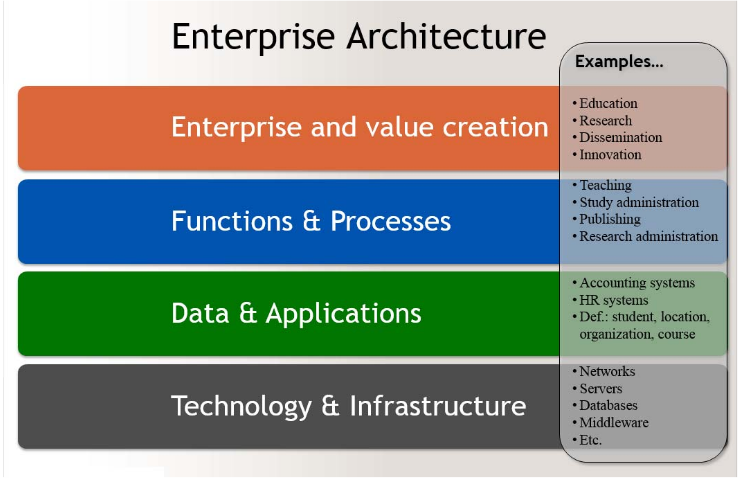
\includegraphics[width=0.75\textwidth]{Abbildungen/ICT_NO.png}
\caption{Vereinfachte Version des TOGAF-Modells für EA nach \autocite{ICT2015}}
\label{fig:TOGAF}
\end{center}
\end{figure}

Das Modell ist eine vereinfachte Form des TOGAF9-Modells, das in Norwegen weit verbreitet ist. Abgebildet ist wie verschiedene Schichten oder Schichten inUnternehmen interagieren, um hohe Qualität, relevante Lösungen und gute Interaktion auf der ganzen Linie zu gewährleisten.

Im Jahr 2016 wurde vom norwegischen Ministerium für Bildung und Forschung eine Umfrage durchgeführt, bei der IT-Mitarbeiter im Interview Fragen zum Einsatz von EA beantworten mussten \autocite{Olsen2016}. Die Ergebnisse der Umfrage werden im Folgenden beschrieben und in \autoref{tab:UniversitiesNO} dargestellt.
% Tabelle
\begin{table}[htbp]
\caption{Institutionen und Informanten \autocite{Olsen2016}}
\begin{center}
\begin{tabularx}{\textwidth}{|p{5cm}|p{3cm}|X|X|X|}
\hline
Institution										& Größe									& \mbox{Größe der} \mbox{IT-Abteilung}	& Anzahl der Informanten	& Interviews \\\hline
University of Agder								& 11.000 Studenten 950 Mitarbeiter		& 60						& 2 						& 3 \\\hline
University of Oslo								& 27.000 Studenten 6.000 Mitarbeiter	& 200						& 1							& 1 \\\hline
Norwegian University \mbox{of Science and Technology}	& 23.000 Studenten 5.000 Mitarbeiter	& 160						& 2 						& 2 \\\hline
University of Nordland							& 6.500 Studenten 650 Mitarbeiter		& 15						& 1 						& 1 \\\hline
University of Troms\o							& 11.800 Studenten 2.900 Mitarbeiter	& 130 						& 1 						& 1 \\\hline
Telemark University College						& 6.500 Studenten 650 Mitarbeiter 		& 20 						& 1 						& 1 \\\hline
Oslo and Akershus University College			& 16.500 Studenten 1.850 Mitarbeiter	& 90 						& 1 						& 1 \\\hline
Narvik University College						& 1.850 Studenten 200 Mitarbeiter 		& 7							& 1 						& 1 \\\hline
Gemeinesammes Verwaltungsdienstleistungszentrum	& 85 Mitarbeiter 						& -		 					& 1 						& 1 \\\hline
\end{tabularx}
\end{center}
\label{tab:UniversitiesNO}
\end{table}%


Während es Meinungsverschiedenheiten zwischen dem Ministerium und den Institutionen über die Verantwortlichkeit und Kostenzuordnung gab, hatte das Architektur-Gremium noch keine Umfrage erstellt. Als Ergebnis hat kein Unternehmen ein formales Mandat auf den Weg gebracht.

Viele Arbeiten werden regelmäßig und funktional durchgeführt, aber ohne eine klare gemeinsame Vision. Einige der Institutionen haben Gruppen oder Abteilungen, die mit EA arbeiten, während andere diese nicht haben. Viele der Befragten gaben an, dass der Sektor noch etwas unreif sei, sowohl im Top-Management als auch auf tieferenOrganisationsebenen.
Schlussfolgerungen

Die Befragten haben angenommen, dass große Universitäten es gut verwalten, aber  kleine Hochschulen waren bei der Umsetzung sorglos. Einige Befragte wurden darauf hingewiesen, dass kleine Institute kleine IT-Abteilungen haben, und dass sie zu beschäftigt mit dem täglichen Betrieb waren. Daher sei es sehr schwierig, den Fokus auf eine strategischen Ebene zu legen. Einige Informanten glaubten auch, dass es auf die Technik zu viel Fokus ist nicht auf architektonische Geschäft. Sie glauben auch, dass es Vorteile in Form von niedrigeren Ausgaben bringt, dass es die Dinge vereinfachen wird,

Auf die Frage \glqq Glauben Sie, dass, wenn die Verfahren für den gesamten Sektor standardisiert sind, Institutionen viel besser gemeinsame Systemanforderungen schaffen können?\grqq 
kommentierte ein fünfter Befragter:
\glqq Ein Teil des Problems ist, dass wir zu klein sind und keinen Einfluss haben, aber wenn wir einige grundlegende Prinzipien hätten, könnten wir diese anwenden.\grqq

Die vorgeschlagenen architektonischen Prinzipien sind nur  Ratschläge. Viele Menschen nahmen TOGAF Kurse und Informanten empfinden es als nützlichen Rahmen. Während es Meinungsverschiedenheiten zwischen dem Ministerium und den Institutionen über die Verantwortlichkeit und Kostenzuordnung gab, hatte das Architektur-Gremium noch keineUmfrage erstellt. Als Ergebnis hat kein Unternehmen ein formales Mandat auf den Weg gebracht.

Viele Aufgaben werden regelmäßig und funktional erledigt, aber ohne eine klare gemeinsame Vision. Einige der Institutionen haben Gruppen oder Abteilungen, die die EA Vision verfolgen, und andere nicht. Es ist auch ein großes Problem, dass das Konzept von EA nicht gut von den Top-Managern verstaden wird und deshalb nicht richtig den IT-Mitarbeitern weitergegeben wird. 


\section{Fazit}
% 400 Wörter / 1S
% Ein Satz?
\begin{APAitemize}
\item EAM findet sich hauptsächlich in großen Unternehmen.
\item Mit der Einbindung von EAM können sowohl in Entscheidungsprozessen als auch in den Routineaufgaben ganz natürliche Veränderungen erreicht werden.
\item Ein CIO sollte die richtigen Leute auswählen, um ein Team zu gründen.
\item Die Geschäftsarchitektur der Bank kann helfen, verschiedene Bankverwaltungssysteme aufzubauen.
\item BIAN Framework bietet eine gute Architektur, aber es ist teuer und die Unternehmen müssen ihre Unternehmen unterstützen.
\item Die Anwendung der EA könnte die Qualität öffentlicher Dienste verbessern. \item Die NEA von Dänemark basiert auf den einzelnen Planungsprozessen, aber die Niederländische NEA besteht aus einer Reihe von Prinzipien und Richtlinien.
\item Die Einführung einer EA im Bildungssystem ist schwierig. Die Befragten in Norwegen antworteten, dass es keine Bereitschaft gibt, sowohl in der Geschäftsleitung als auch auf organisatorischer Ebene.
\item Im Vergleich dazu ist es einfacher, EA im privaten Sektor (Unternehmen, Banken) anstatt im öffentlichen Sektor (Bildung und Regierung) zu integrieren.
\end{APAitemize}
% Ein Satz?

\newpage

\printbibliography

\end{document}  